Once he gets to the Whispering Gallery, Jorge realizes that the girl was
right. This \emph{is} the center of the universe. There are murmurs to
be heard there -- it seems they come from everywhere. He hears about
guilds and the craftsmen who built the cathedral. He learns about how
proud they were and how they formed communities of practice, educating
the uninitiated, teaching each other to create. He returns to ground
level. The girl is gone, but he feels happy and inspired.~ He can do
much more then repackage social media streams; there is more going on
here than Twitter as a new broadcast medium.~ He starts a new journey:
finding a guild, a community of practice, but restyled in a 21st century
fashion.~ It will be more open, more connected to others then the old
guilds. He will still use Twitter, a social dashboard, and curating
tools, but also he uses wikis, and synchronous communication.~ And most
importantly, he starts building, together with others -- in particular,
together with the people formerly known as his readers. They will
co-create the analysis, the search for solutions and sense-making,
rather than helplessly listening to ``experts'', passively consuming
pre-processed knowledge and information. Instead, they'll start building
their own destiny, and the newsroom will be part of the platform.
{[}caption id=``'' align=``aligncenter''
width=``520''{]}\href{http://peeragogy.org/a-story-of-beginnings/section/}{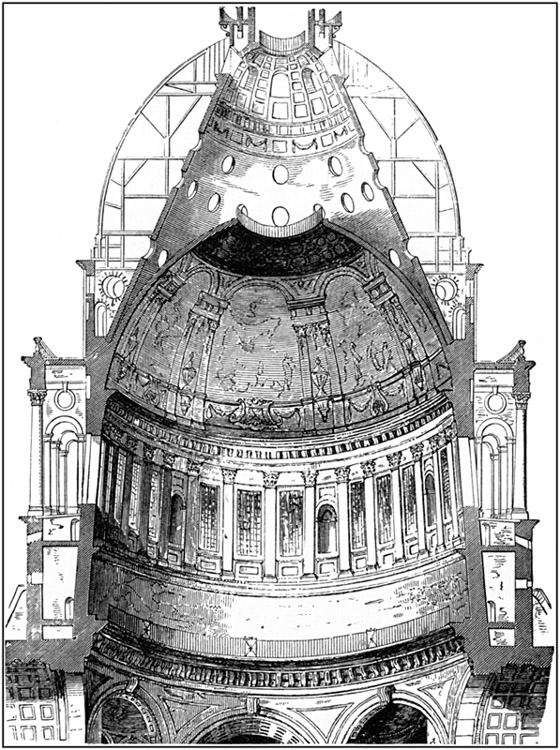
\includegraphics{http://peeragogy.org/wp-content/uploads/2013/12/section.jpg}}
Section of the Dome at St Paul's Cathedral{[}/caption{]}
